% Created 2014-09-11 Thu 15:11
\documentclass[table,smaller]{beamer}
\usepackage[utf8]{inputenc}
\usepackage[T1]{fontenc}
\usepackage{fixltx2e}
\usepackage{graphicx}
\usepackage{longtable}
\usepackage{float}
\usepackage{wrapfig}
\usepackage{rotating}
\usepackage[normalem]{ulem}
\usepackage{amsmath}
\usepackage{textcomp}
\usepackage{marvosym}
\usepackage{wasysym}
\usepackage{amssymb}
\usepackage{hyperref}
\tolerance=1000
\usepackage{tikz}
\usepackage{minted}
\usepackage{fancyvrb}
\usemintedstyle{perldoc}
\definecolor{lightgray}{gray}{0.96}
\setlength{\tabcolsep}{1ex}
\usetheme{Warsaw}
\useoutertheme{infolines}
\setbeamercolor{block body}{bg=lightgray}
\titlegraphic{
\includegraphics[width=.75\textwidth]{images/IQSSNewLogo.pdf}}
\setbeamersize{text margin left=2em,text margin right=2em}
\AtBeginSection[]{\begin{frame}<beamer>\frametitle{Topic}\tableofcontents[currentsection]\end{frame}}
\usetheme{default}
\author{Ista Zahn}
\date{}
\title{Introduction to R}
\hypersetup{
  pdfkeywords={},
  pdfsubject={},
  pdfcreator={Emacs 24.3.1 (Org mode 8.2.7c)}}
\begin{document}

\maketitle
\begin{frame}{Outline}
\tableofcontents
\end{frame}



\section{Workshop Materials and Introduction}
\label{sec-1}

\begin{frame}[label=sec-1-1]{Materials and setup}
Everyone should have R installed --if not:

\begin{itemize}
\item Open a web browser and go to \url{http://cran.r-project.org} and download and install it
\item Also helpful to install RStudo (download from \url{http://rstudio.com})
\end{itemize}

Materials for this workshop include slides, example data sets, and example code.

\begin{itemize}
\item Download materials from \url{http://tutorials.iq.harvard.edu/R/Rintro.zip}
\item Extract the zip file containing the materials to your desktop
\end{itemize}

Workshop notes are available in .hmtl and .pdf format. Navigate to your desktop and open either Rintro.pdf or Rintro.html.
\end{frame}


\begin{frame}[label=sec-1-2]{What is R?}
R is a programming language designed for statistical computing. Notable characteristics include:

\begin{itemize}
\item Vast capabilities, wide range of statistical and graphical techniques

\item Very popular in academia, growing popularity in business: \url{http://r4stats.com/articles/popularity/}

\item Written primarily by statisticians

\item FREE (no cost, open source)

\item Excellent community support: mailing list, blogs, tutorials

\item Easy to extend by writing new functions
\end{itemize}
\end{frame}

\begin{frame}[label=sec-1-3]{Coming to R}
Comming from\ldots{}
{\footnotesize
\begin{description}
\item[{Stata}] \url{http://www.princeton.edu/~otorres/RStata.pdf}
\item[{SAS/SPSS}] \url{http://www.et.bs.ehu.es/~etptupaf/pub/R/RforSAS&SPSSusers.pdf}
\item[{matlab}] \url{http://www.math.umaine.edu/~hiebeler/comp/matlabR.pdf}
\item[{Python}] \url{http://mathesaurus.sourceforge.net/matlab-python-xref.pdf}
\end{description}
}
\end{frame}

\section{Graphical User Interfaces}
\label{sec-2}


\begin{frame}[label=sec-2-1]{R GUI alternatives (no GUI)}
The old-school way is to run R directly in a terminal

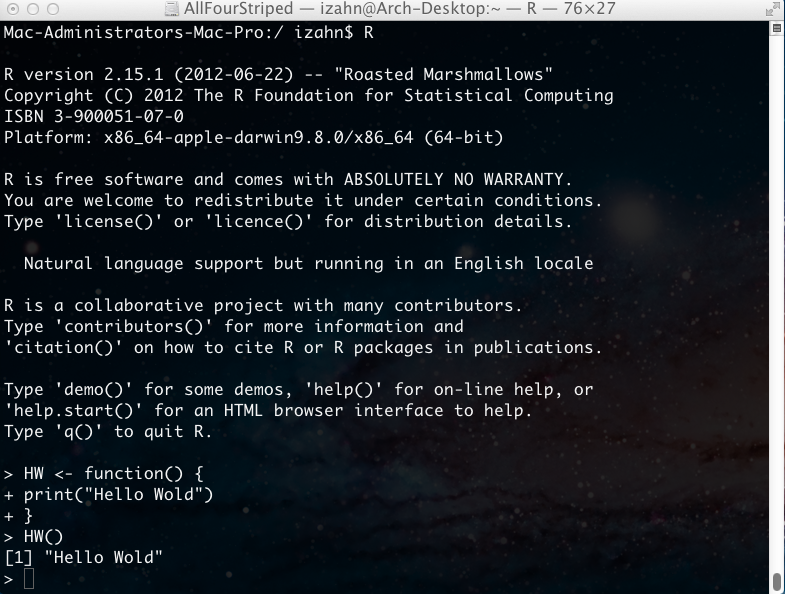
\includegraphics[width=.75\textwidth]{images/Rconsole.png}

But hardly anybody does it that way anymore!
\end{frame}


\begin{frame}[label=sec-2-2]{R GUI alternatives (Windows default)}
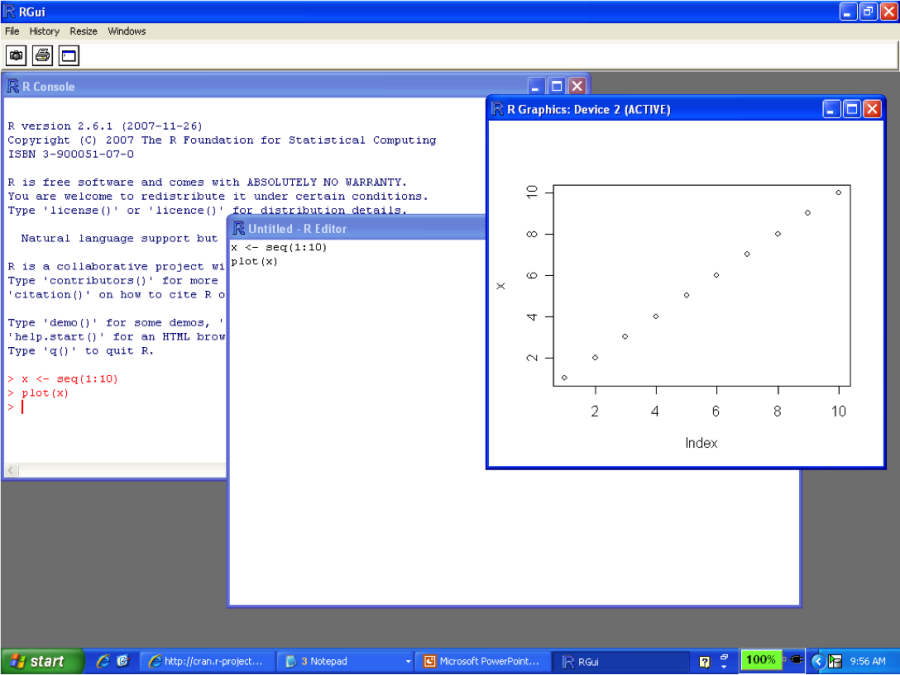
\includegraphics[width=.75\textwidth]{images/Rgui.png}

The default windows GUI is not very good
\begin{itemize}
\item No parentheses matching or syntax highlighting
\item No work-space browser
\end{itemize}
\end{frame}


\begin{frame}[label=sec-2-3]{R GUI Alternatives (Rstudio on Mac)}
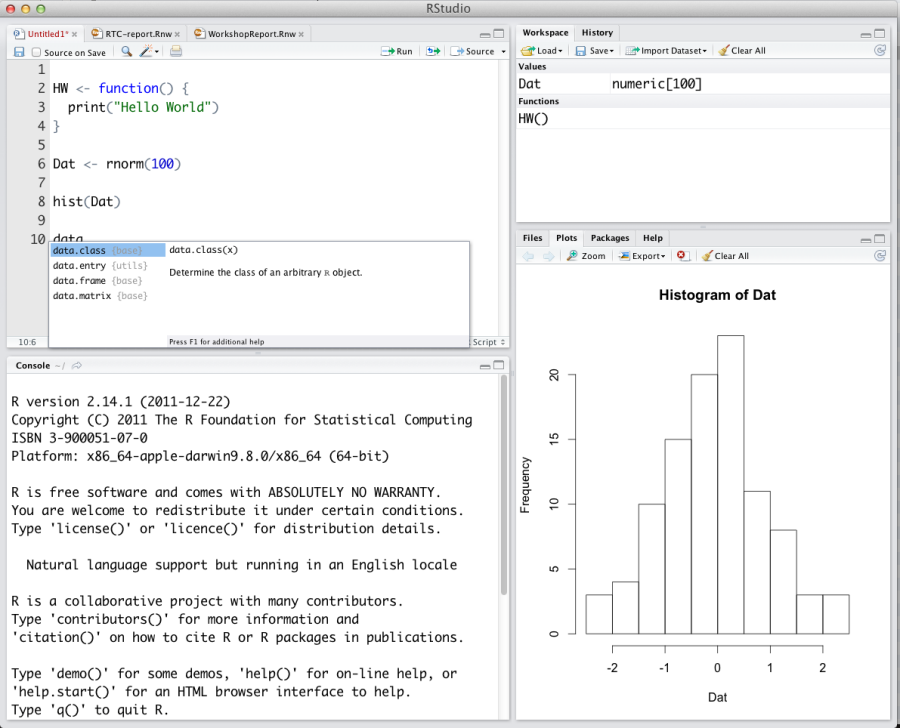
\includegraphics[width=.75\textwidth]{images/Rstudio.png}

Rstudio has many useful features, including parentheses matching and auto-completion
\end{frame}


\begin{frame}[label=sec-2-4]{R GUI Alternatives (Emacs with ESS)}
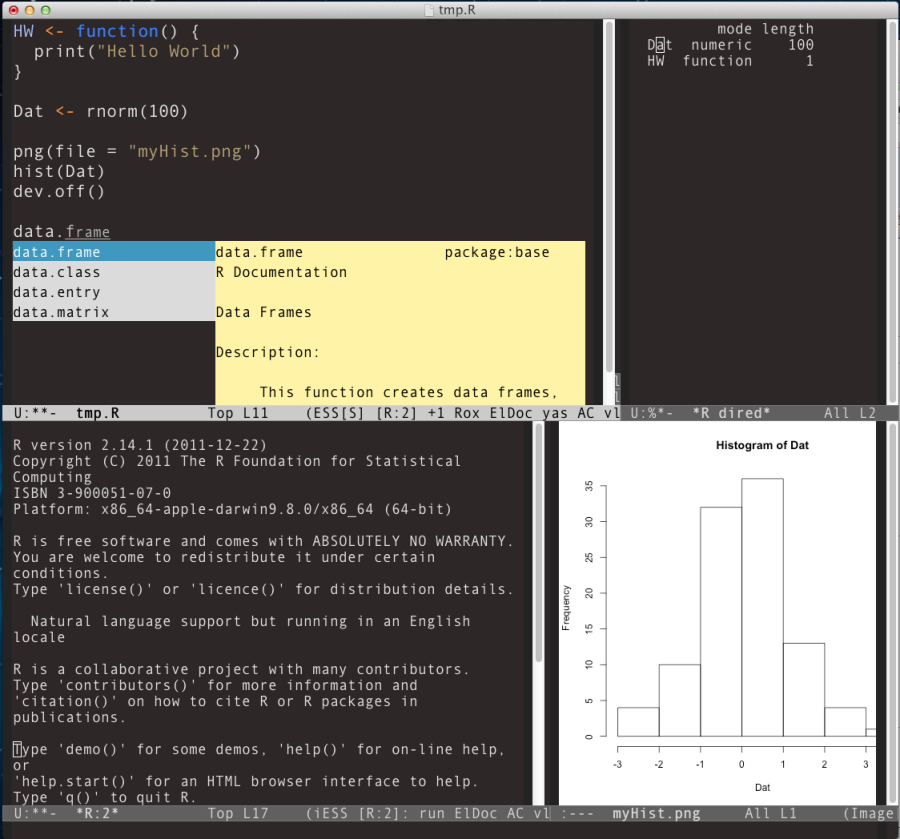
\includegraphics[width=.65\textwidth]{images/emacs.png}

Emacs + ESS is a very powerful combination, but can be difficult to set up
\end{frame}


\begin{frame}[fragile,label=sec-2-5]{Launch RStudio}
 \begin{itemize}
\item Open the RStudio program

\item Open up today's R script

\begin{itemize}
\item In RStudio, Go to \alert{File => Open Script}

\item Locate and open the \texttt{Rintro.R} script in the Rintro folder on your desktop
\end{itemize}

\item Go to \alert{Tools => Set working directory => To source file location} (more on the working directory later)

\item I encourage you to add your own notes to this file!
\end{itemize}
\end{frame}

\begin{frame}[fragile,label=sec-2-6]{Things to keep in mind}
 \begin{itemize}
\item Case sensitive, like Stata (unlike SAS)

\item Comments can be put almost anywhere, starting with a hash mark ('\texttt{\#}'); everything to the end of the line is a comment

\item The command prompt "\texttt{>}" indicates that R is ready to receive commands

\item If a command is not complete at the end of a line, R will give a different prompt, '\texttt{+}' by default

\item Parentheses must always match (first thing to check if you get an error)

\item R Does not care about spaces between commands or arguments

\item Names should start with a letter and should not contain spaces

\item Can use "." in object names (e.g., "my.data")

\item Use forward slash ("/") instead of backslash in path names, even on Windows
\end{itemize}
\end{frame}


\begin{frame}[label=sec-2-7]{Exercise 0}
\begin{enumerate}
\item Try to get R to add 2 plus 2.
\item Try to figure out how evaluate lines directly from your R script.
\item R includes extensive documentation, including a file named "An introduction to R". Try to find this help file.
\item Go to \url{http://cran.r-project.org/web/views/} and skim the topic closest to your field/interests.
\end{enumerate}
\end{frame}


\section{Data and Functions}
\label{sec-3}

\begin{frame}[fragile,label=sec-3-1]{Assignment}
 Values can be assigned names and used in subsequent operations
\begin{itemize}
\item The \verb~<-~ operator (less than followed by a dash) is used to save values
\item The name on the left gets the value on the right.
\end{itemize}

\vspace{-.5em}
\begin{columns}
\column{.95\linewidth}
\begin{block}{}
\begin{minted}[linenos=false, fontsize=\footnotesize]{rconsole}
> x <- 11 # Assign the value 10 to a variable named x
> x + 1 # Add 1 to x
[1] 12
> y <- x + 1 # Assign y the value x + 1
> y
[1] 12
>
\end{minted}
\end{block}
\end{columns}
\vspace{.5em}


Saved variables can be listed, overwritten and deleted
\vspace{-.5em}
\begin{columns}
\column{.95\linewidth}
\begin{block}{}
\begin{minted}[linenos=false, fontsize=\footnotesize]{rconsole}
> ls() # List variables in workspace
[1] "x" "y"
> x # Print the value of x
[1] 11
> x <- 100 # Overwrite x. Note that no warning is given!
> x
[1] 100
> rm(x) # Delete x
> ls()
[1] "y"
>
\end{minted}
\end{block}
\end{columns}
\vspace{.5em}
\end{frame}


\begin{frame}[fragile,label=sec-3-2]{Functions}
 Using R is mostly about applying \alert{functions} to \alert{variables}. Functions
\begin{itemize}
\item take \alert{variable(s)} as input \alert{argument(s)}
\item perform operations
\item \alert{return} values which can be \alert{assigned}
\item optionally perform side-effects such as writing a file to disk or opening a graphics window
\end{itemize}

The general form for calling R functions is 
\begin{minted}[fontsize=\scriptsize]{r}
FunctionName(arg.1, arg.2, ... arg.n)
\end{minted}

Arguments can be matched by position or name

Examples:
\vspace{-.5em}
\begin{columns}
\column{.95\linewidth}
\begin{block}{}
\begin{minted}[linenos=false, fontsize=\footnotesize]{rconsole}
> #?sqrt
> a <- sqrt(y) # Call the sqrt function with argument x=y
> round(a, digits = 2) # Call round() with arguments x=x and digits=2
[1] 3.46
> # Functions can be nested so an alternative is
> round(sqrt(y), digits = 5) # Take sqrt of a and round
[1] 3.4641
>
\end{minted}
\end{block}
\end{columns}
\vspace{.5em}
\end{frame}


\section{Help and package management}
\label{sec-4}

\begin{frame}[fragile,label=sec-4-1]{Asking R for help}
 R has extensive built-in documentation that can be accessed through R commands or through the GUI.
\begin{itemize}
\item Start html help, search/browse using web browser
\begin{itemize}
\item at the R console:
\begin{minted}[fontsize=\scriptsize]{r}
help.start()
\end{minted}

\item or use the help menu from you GUI
\end{itemize}

\item Look up the documentation for a function
\begin{minted}[fontsize=\scriptsize]{r}
help(plot)
\end{minted}

\begin{minted}[fontsize=\scriptsize]{r}
?kmeans
\end{minted}

\item Look up documentation for a package
\begin{minted}[fontsize=\scriptsize]{r}
help(package="stats")
\end{minted}

\item Search documentation from R (not always the best way\ldots{} google often works better)
\begin{minted}[fontsize=\scriptsize]{r}
help.search("classification")
\end{minted}
\end{itemize}
\end{frame}

\begin{frame}[fragile,label=sec-4-2]{R packages and libraries}
 There are thousands of R packages that extend R's capabilities.

\begin{itemize}
\item To view available packages: 
\begin{minted}[fontsize=\scriptsize]{r}
library()
\end{minted}

\item To see what packages are loaded: 
\begin{minted}[fontsize=\scriptsize]{r}
search()
\end{minted}

\item To load a package: 
\begin{minted}[fontsize=\scriptsize]{r}
library("car")
\end{minted}

\item Install new package: 
\begin{minted}[fontsize=\scriptsize]{r}
install.packages("stringdist")
\end{minted}
\end{itemize}
\end{frame}


\section{Getting data into R}
\label{sec-5}


\begin{frame}[fragile,label=sec-5-1]{The gss dataset}
 The next few examples use a subset of the General Social Survey data set. The variables in this subset include
\vspace{-.5em}
\begin{columns}
\column{.95\linewidth}
\begin{block}{}
\begin{minted}[linenos=false, fontsize=\footnotesize]{rconsole}
> head(read.csv("dataSets/gssInfo.csv")) 
      var                      description
1 marital                   marital status
2     age                age of respondent
3    educ highest year of school completed
4     sex                  respondents sex
5     inc               respondents income
6   happy                general happiness
> #see gssInfo.csv for rest of the variable descriptions
>
\end{minted}
\end{block}
\end{columns}
\vspace{.5em}
\end{frame}

\begin{frame}[fragile,label=sec-5-2]{The "working directory" and listing files}
  R knows the directory it was started in, and refers to this as the "working directory". Since our workshop examples are in the Rintro folder on the desktop, we should all take a moment to set that as our working directory:
We can also set the working directory using paths relative to the current working directory:

\vspace{-.5em}
\begin{columns}
\column{.95\linewidth}
\begin{block}{}
\begin{minted}[linenos=false, fontsize=\footnotesize]{rconsole}
> getwd() # get the current working directory
[1] "/home/izahn/Documents/Work/IQSS/Classes/IQSS_Stats_Workshops/R/Rintro"
> setwd("dataSets") # set wd to the dataSets folder
> getwd()
[1] "/home/izahn/Documents/Work/IQSS/Classes/IQSS_Stats_Workshops/R/Rintro/dataSets"
> setwd("..") # set wd to enclosing folder ("up")
>
\end{minted}
\end{block}
\end{columns}
\vspace{.5em}

It can be convenient to list files in a directory without leaving R
\vspace{-.5em}
\begin{columns}
\column{.95\linewidth}
\begin{block}{}
\begin{minted}[linenos=false, fontsize=\footnotesize]{rconsole}
> list.files("dataSets") # list files in the dataSets folder
 [1] "gss.csv"            "gss.dta"            "gssInfo.csv"       
 [4] "gss.rds"            "gss.sas7bdat"       "gss.sav"           
 [7] "gss.xlsx"           "statesCodebook.txt" "states.csv"        
[10] "states.dta"         "states.xlsx"       
> # list.files("dataSets", pattern = ".csv") # restrict to .csv files  
>
\end{minted}
\end{block}
\end{columns}
\vspace{.5em}
\end{frame}


\begin{frame}[fragile,label=sec-5-3]{Importing data from files}
 In order to read data from a file, you have to know what kind of file it is. The table below lists the functions needed to import data from common file formats.

\begin{center}
\begin{tabular}{lll}
data type & function & package\\
\hline
comma separated (.csv) & read.csv() & utils (default)\\
other delimited formats & read.table() & utils (default)\\
Stata (.dta) & read.dta() & foreign\\
SPSS (.sav) & read.spss() & foreign\\
SAS (.sas7bdat) & read.sas7bdat() & sas7bdat\\
Excel (.xls, .xlsx) & readWorksheetFromFile() & XLConnect\\
\hline
\end{tabular}
\end{center}

Examples:
\vspace{-.5em}
\begin{columns}
\column{.95\linewidth}
\begin{block}{}
\begin{minted}[linenos=false, fontsize=\footnotesize]{rconsole}
> # read gss data from the gss.rds R file
> datGSS <- readRDS("dataSets/gss.rds")
> # read gss data from the gss.csv comma separated file
> gss.data <- read.csv("dataSets/gss.csv") # read gss data
> # read a Stata dataset from gss.dta 
> library(foreign) # load foreign data functions
> datGSS <- read.dta(file="dataSets/gss.dta")
>
\end{minted}
\end{block}
\end{columns}
\vspace{.5em}
\end{frame}


\begin{frame}[fragile,label=sec-5-4]{Checking imported data}
 Always a good idea  to examine the imported data set--usually we want the results to be a \verb~data.frame~
\vspace{-.5em}
\begin{columns}
\column{.95\linewidth}
\begin{block}{}
\begin{minted}[linenos=false, fontsize=\footnotesize]{rconsole}
> class(datGSS) # check to see that test is what we expect it to be
[1] "data.frame"
> dim(datGSS) # how many rows and columns?
[1] 1419   35
> names(datGSS)[1:10] # first 10 column names
 [1] "age"      "educ"     "emailhrs" "hrs1"     "sex"      "usecomp" 
 [7] "usemail"  "useweb"   "webhrs"   "hapmar"  
> str(datGSS[1:5]) # more details about the first 5 columns
'data.frame':	1419 obs. of  5 variables:
 $ age     : num  69 27 19 21 19 87 42 19 78 70 ...
 $ educ    : num  12 10 11 9 11 8 11 11 7 9 ...
 $ emailhrs: num  -1 -1 0 -1 50 -1 3 -1 -1 -1 ...
 $ hrs1    : num  -1 60 32 20 -1 -1 -1 -1 -1 22 ...
 $ sex     : Factor w/ 2 levels "Male","Female": 1 1 1 1 1 2 1 2 2 2 ...
>
\end{minted}
\end{block}
\end{columns}
\vspace{.5em}
\end{frame}


\begin{frame}[fragile,label=sec-5-5]{Saving and loading R  workspaces}
 In addition to importing individual datasets, R can save and load entire workspaces
\begin{itemize}
\item Save our entire workspace
\end{itemize}
\vspace{-.5em}
\begin{columns}
\column{.95\linewidth}
\begin{block}{}
\begin{minted}[linenos=false, fontsize=\footnotesize]{rconsole}
> ls() # list objects in our workspace
[1] "a"        "datGSS"   "gss.data" "y"       
> save.image(file="myWorkspace.RData") # save workspace 
> rm(list=ls()) # remove all objects from our workspace 
> ls() # list stored objects to make sure they are deleted
character(0)
>
\end{minted}
\end{block}
\end{columns}
\vspace{.5em}

\begin{itemize}
\item Load the "myWorkspace.RData" file and check that it is restored
\end{itemize}

\vspace{-.5em}
\begin{columns}
\column{.95\linewidth}
\begin{block}{}
\begin{minted}[linenos=false, fontsize=\footnotesize]{rconsole}
> load("myWorkspace.RData") # load myWorkspace.RData
> ls() # list objects
[1] "a"        "datGSS"   "gss.data" "y"       
>
\end{minted}
\end{block}
\end{columns}
\vspace{.5em}

When you close R you will be asked if you want to save your workspace -- if you choose yes then your workspace will be restored next time you start R
\end{frame}


\begin{frame}[label=sec-5-6]{Exercise 1}
\begin{enumerate}
\item Load the foreign package if you haven't already done so

\item Look at the help page for the read.spss function

\item Read the SPSS data set in dataSets/gss.sav and assign the result to an R data object named GSS.sav

\item Make sure that the data loaded in step 2 is a data.frame (hint: check the arguments documented in the help page)

\item Display the dimensions of the GSS.sav.

\item BONUS: figure out how to read the Excel file "gss.xlsx" into R
\end{enumerate}
\end{frame}


\section{Data Manipulation}
\label{sec-6}

\begin{frame}[label=sec-6-1]{data.frame objects}
\begin{itemize}
\item Usually data read into R will be stored as a \alert{data.frame}

\item A data.frame is a list of vectors of equal length
\begin{itemize}
\item Each vector in the list forms a column
\item Each column can be a differnt type of vector
\item Often the columns are variables and the rows are observations
\end{itemize}

\item A data.frame has two dimensions corresponding the number of rows and the number of columns (in that order)
\end{itemize}
\end{frame}

\begin{frame}[fragile,label=sec-6-2]{data.frame meta-data}
 A number of functions are available for inspecting data.frame objects:

\vspace{-.5em}
\begin{columns}
\column{.95\linewidth}
\begin{block}{}
\begin{minted}[linenos=false, fontsize=\footnotesize]{rconsole}
> # row and column names
> head(names(datGSS)) # variable names in datGSS
[1] "age"      "educ"     "emailhrs" "hrs1"     "sex"      "usecomp" 
> head(rownames(datGSS)) # first few rownames of datGSS
[1] "1" "2" "3" "4" "5" "6"
> # dimensions
> dim(datGSS)
[1] 1419   35
> # structure
> #str(datGSS) # get structure
>
\end{minted}
\end{block}
\end{columns}
\vspace{.5em}
\end{frame}


\begin{frame}[label=sec-6-3]{Logical operators}
It is often useful to select just those rows of your data where some condition holds--for example select only rows where sex is 1 (male). The following operators allow you to do this:

\begin{description}
\item[{==}] equal to
\item[{!=}] not equal to
\item[{>}] greater than
\item[{<}] less than
\item[{>=}] greater than or equal to
\item[{<=}] less than or equal to
\item[{\&}] and
\item[{|}] or
\end{description}

Note the double equals signs for testing equality. The following example show how to use some of these operators to extract and replace elements matching specific conditions.
\end{frame}


\begin{frame}[fragile,label=sec-6-4]{Extracting subsets of data.frames}
 You can extract subsets of data.frames using the \texttt{subset()} function.

\vspace{-.5em}
\begin{columns}
\column{.95\linewidth}
\begin{block}{}
\begin{minted}[linenos=false, fontsize=\footnotesize]{rconsole}
> # extracting subsets
> subset(datGSS,
+        # rows 1 through 3
+        subset = rownames(datGSS) %in% 1:3,
+        # column 1 to 5
+        select = 1:4)
  age educ emailhrs hrs1
1  69   12       -1   -1
2  27   10       -1   60
3  19   11        0   32
>                                         
> subset(datGSS,
+        # rows where age > 90
+        subset = age > 90,
+        ## sex and age columns
+        select = c("sex", "age"))
       sex age
315 Female  99
665   Male  99
> 
> ## the $ operator can be used to extract a single column
> str(datGSS$age)
 num [1:1419] 69 27 19 21 19 87 42 19 78 70 ...
>
\end{minted}
\end{block}
\end{columns}
\vspace{.5em}

Note that \texttt{subset()} is a convenience function; see \texttt{?Extract} for a more powerful (and complicated) way to subset data.
\end{frame}

\begin{frame}[fragile,label=sec-6-5]{Transforming data.frames}
 You can modify data.frames using the \texttt{transform()} function. 

\vspace{-.5em}
\begin{columns}
\column{.95\linewidth}
\begin{block}{}
\begin{minted}[linenos=false, fontsize=\footnotesize]{rconsole}
> # creating new variable mean centered age
> datGSS <- transform(datGSS,
+                     ageC = age - mean(age))
> 
>  #education difference between wifes and husbands
> datGSS <- transform(datGSS,
+                     educ.diff = wifeduc - husbeduc)
> 
> ## ifelse() is also useful; note that the $ operator can
> ## also be used to create new variables.
> datGSS$young <- ifelse(datGSS$age < 30, "yes", "no")
> 
> ## examine our newly created variables
> head(subset(datGSS,
+             select = c("age", "ageC", "young", "wifeduc",
+                        "husbeduc", "educ.diff")),
+      n = 8)
  age       ageC young wifeduc husbeduc educ.diff
1  69  22.363636    no      NA       NA        NA
2  27 -19.636364   yes      13       10         3
3  19 -27.636364   yes      NA       NA        NA
4  21 -25.636364   yes      NA       NA        NA
5  19 -27.636364   yes      NA       NA        NA
6  87  40.363636    no      NA       NA        NA
7  42  -4.636364    no      10       11        -1
8  19 -27.636364   yes      NA       NA        NA
>
\end{minted}
\end{block}
\end{columns}
\vspace{.5em}

Note that \texttt{transform} is a convenience function; see \texttt{?Extract} for a more powerful way to modify data.frames.
\end{frame}

\begin{frame}[fragile,label=sec-6-6]{Exporting Data}
 Now that we have made some changes to our GSS data set, we might want to save those changes to a file. Everything we have done so far has only modified the data in R; the files have remained unchanged. 

\vspace{-.5em}
\begin{columns}
\column{.95\linewidth}
\begin{block}{}
\begin{minted}[linenos=false, fontsize=\footnotesize]{rconsole}
> # write data to a .csv file
> write.csv(datGSS, file = "gss.csv")
> # write data to a Stata file
> write.dta(datGSS, file = "gss.dta")
> # write data to an R file
> saveRDS(datGSS, file = "gss.rds")
>
\end{minted}
\end{block}
\end{columns}
\vspace{.5em}
\end{frame}


\begin{frame}[label=sec-6-7]{Exercise 2: Data manipulation}
Use the gss.rds data set

\begin{enumerate}
\item Generate the following variables:
\begin{itemize}
\item "rich" equal to 0 if rincdol is less than 100000, and 1 otherwise
\item "sinc" equal to incomdol - rincdol
\end{itemize}
\item Create a subset of the data containing only rows where "usecomp" = "Yes"
\item Examine the data.frame created in step 2, and answer the following questions:
\begin{itemize}
\item How many rows does it have?
\item How many columns does it have?
\item What is the class of the "satjob" variable?
\end{itemize}
\item BONUS (hard): Generate a variable named "dual.earn" equal to 1 if both wkftwife = 1 and wkfthusb = 1, and zero otherwise
\end{enumerate}
\end{frame}



\section{Basic Statistics and Graphs}
\label{sec-7}

\begin{frame}[fragile,label=sec-7-1]{Basic statistics}
 Descriptive statistics of single variables are straightforward:
\vspace{-.5em}
\begin{columns}
\column{.95\linewidth}
\begin{block}{}
\begin{minted}[linenos=false, fontsize=\footnotesize]{rconsole}
> mean(datGSS$educ) # calculate mean value of education
[1] 13.47498
> sd(datGSS$educ) # calculate standard deviation of x
[1] 5.389476
> # calculate min, max, quantiles, mean of educ, age, and ageC
> summary(subset(datGSS, select = c("educ", "age", "ageC")))
      educ            age             ageC        
 Min.   : 0.00   Min.   :18.00   Min.   :-28.636  
 1st Qu.:12.00   1st Qu.:32.00   1st Qu.:-14.636  
 Median :13.00   Median :44.00   Median : -2.636  
 Mean   :13.47   Mean   :46.64   Mean   :  0.000  
 3rd Qu.:16.00   3rd Qu.:59.00   3rd Qu.: 12.364  
 Max.   :99.00   Max.   :99.00   Max.   : 52.364  
>
\end{minted}
\end{block}
\end{columns}
\vspace{.5em}


Some of these functions (e.g., summary) will also work with data.frames and other types of objects, others (such as \texttt{sd}) will not.
\end{frame}

\begin{frame}[fragile,label=sec-7-2]{Counts and proportions}
 Start by using the \verb~table()~ function to tabulate counts, then perform additional computations if needed
\vspace{-.5em}
\begin{columns}
\column{.95\linewidth}
\begin{block}{}
\begin{minted}[linenos=false, fontsize=\footnotesize]{rconsole}
> sex.counts <- table(datGSS$sex) # tabulate sex categories
> sex.counts

  Male Female 
   622    797 
> prop.table(sex.counts) # convert to proportions

     Male    Female 
0.4383369 0.5616631 
>
\end{minted}
\end{block}
\end{columns}
\vspace{.5em}

Add variables for crosstabs

\vspace{-.5em}
\begin{columns}
\column{.95\linewidth}
\begin{block}{}
\begin{minted}[linenos=false, fontsize=\footnotesize]{rconsole}
> table(subset(datGSS, select = c("sex", "happy"))) # crosstab marital X happy
        happy
sex      NAP VERY HAPPY PRETTY HAPPY NOT TOO HAPPY  DK  NA
  Male     0        189          350            73   0  10
  Female   0        246          447            84   1  19
>
\end{minted}
\end{block}
\end{columns}
\vspace{.5em}
\end{frame}



\begin{frame}[fragile,label=sec-7-3]{Statistics by classification factors}
 The \verb~by()~ function can be used to perform a calculation separately for each level of a classifying variable
\vspace{-.5em}
\begin{columns}
\column{.95\linewidth}
\begin{block}{}
\begin{minted}[linenos=false, fontsize=\footnotesize]{rconsole}
> by(subset(datGSS, select = c("income", "educ")),
+    INDICES=datGSS["sex"],
+    FUN=summary)
sex: Male
             income         educ      
 $40000 TO 49999: 59   Min.   : 4.00  
 $50000 TO 59999: 56   1st Qu.:12.00  
 $60000 TO 74999: 49   Median :13.00  
 $35000 TO 39999: 48   Mean   :13.68  
 REFUSED        : 48   3rd Qu.:16.00  
 $110000 OR OVER: 43   Max.   :99.00  
 (Other)        :319                  
---------------------------------------------------- 
sex: Female
             income         educ      
 REFUSED        : 76   Min.   : 0.00  
 $60000 TO 74999: 62   1st Qu.:12.00  
 $40000 TO 49999: 60   Median :12.00  
 $50000 TO 59999: 52   Mean   :13.32  
 $30000 TO 34999: 49   3rd Qu.:15.00  
 $25000 TO 29999: 42   Max.   :99.00  
 (Other)        :456                  
>
\end{minted}
\end{block}
\end{columns}
\vspace{.5em}
\end{frame}

\begin{frame}[fragile,label=sec-7-4]{Correlations}
 Let's look at correlations among between age, income, and education
\vspace{-.5em}
\begin{columns}
\column{.95\linewidth}
\begin{block}{}
\begin{minted}[linenos=false, fontsize=\footnotesize]{rconsole}
> cor(subset(datGSS, select =  c("age", "incomdol", "educ")))
                 age   incomdol        educ
age       1.00000000 -0.1186564 -0.07362454
incomdol -0.11865641  1.0000000  0.21013267
educ     -0.07362454  0.2101327  1.00000000
>
\end{minted}
\end{block}
\end{columns}
\vspace{.5em}


For significance tests, use cor.test()
\vspace{-.5em}
\begin{columns}
\column{.95\linewidth}
\begin{block}{}
\begin{minted}[linenos=false, fontsize=\footnotesize]{rconsole}
> with(datGSS,
+      cor.test(age, educ))

	Pearson's product-moment correlation

data:  age and educ
t = -2.779, df = 1417, p-value = 0.005525
alternative hypothesis: true correlation is not equal to 0
95 percent confidence interval:
 -0.12518333 -0.02166916
sample estimates:
        cor 
-0.07362454 

>
\end{minted}
\end{block}
\end{columns}
\vspace{.5em}
\end{frame}

\begin{frame}[fragile,label=sec-7-5]{Multiple regression}
 Modeling functions generally use the \emph{formula} interface whith DV on left followed by "\textasciitilde{}" followed by predictors--for details see
\begin{minted}[fontsize=\scriptsize]{r}
help("formula")
\end{minted}

\begin{itemize}
\item Predict the number of hours individuals spend on email (emailhrs)
\end{itemize}
\vspace{-.5em}
\begin{columns}
\column{.95\linewidth}
\begin{block}{}
\begin{minted}[linenos=false, fontsize=\footnotesize]{rconsole}
> m1 <- lm(educ ~ sex + age, data = datGSS)
> summary(m1)

Call:
lm(formula = educ ~ sex + age, data = datGSS)

Residuals:
    Min      1Q  Median      3Q     Max 
-13.434  -1.785  -0.688   1.955  86.049 

Coefficients:
             Estimate Std. Error t value Pr(>|t|)
(Intercept) 14.652702   0.425691  34.421  < 2e-16
sexFemale   -0.275235   0.289290  -0.951  0.34156
age         -0.021938   0.008238  -2.663  0.00783

Residual standard error: 5.377 on 1416 degrees of freedom
Multiple R-squared:  0.006056,	Adjusted R-squared:  0.004652 
F-statistic: 4.314 on 2 and 1416 DF,  p-value: 0.01356

>
\end{minted}
\end{block}
\end{columns}
\vspace{.5em}
\end{frame}


\begin{frame}[fragile,label=sec-7-6]{Save R output to a file}
 Earlier we learned how to write a data set to a file. But what if we want to write something that isn't in a nice rectangular format, like the results of our regression model? For that we can use the \verb~sink()~ function:

\vspace{-.5em}
\begin{columns}
\column{.95\linewidth}
\begin{block}{}
\begin{minted}[linenos=false, fontsize=\footnotesize]{rconsole}
> sink(file="output.txt", split=TRUE) # start logging
> print("This is the result from model 1\n")
[1] "This is the result from model 1\n"
> print(summary(m1))

Call:
lm(formula = educ ~ sex + age, data = datGSS)

Residuals:
    Min      1Q  Median      3Q     Max 
-13.434  -1.785  -0.688   1.955  86.049 

Coefficients:
             Estimate Std. Error t value Pr(>|t|)
(Intercept) 14.652702   0.425691  34.421  < 2e-16
sexFemale   -0.275235   0.289290  -0.951  0.34156
age         -0.021938   0.008238  -2.663  0.00783

Residual standard error: 5.377 on 1416 degrees of freedom
Multiple R-squared:  0.006056,	Adjusted R-squared:  0.004652 
F-statistic: 4.314 on 2 and 1416 DF,  p-value: 0.01356

> sink() ## sink with no arguments turns logging off
>
\end{minted}
\end{block}
\end{columns}
\vspace{.5em}
\end{frame}


\begin{frame}[fragile,label=sec-7-7]{Basic graphics: Frequency bars}
 Thanks to classes and methods, you can \verb~plot()~ many  kinds of objects:

\begin{columns} \column{.85\textwidth} \begin{block}{}
\begin{minted}[fontsize=\scriptsize]{r}
plot(datGSS$marital) # Plot a factor
\end{minted}
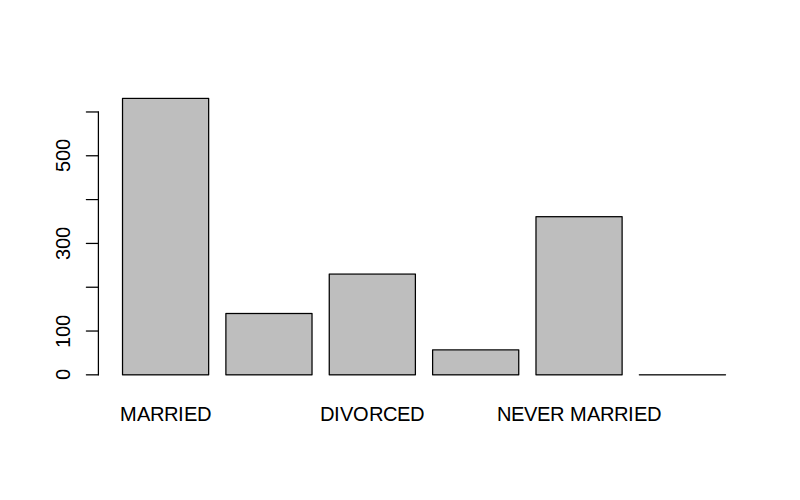
\includegraphics[width=.9\textwidth]{images/examplePlot1.png}



\end{block} \end{columns}
\end{frame}

\begin{frame}[fragile,label=sec-7-8]{Basic graphics: Boxplots by group}
 Thanks to classes and methods, you can \verb~plot()~ many kinds of objects:
\begin{columns} \column{.85\textwidth} \begin{block}{}
\begin{minted}[fontsize=\scriptsize]{r}
with(datGSS,
     plot(marital, educ)) # Plot ordinal by numeric
\end{minted}
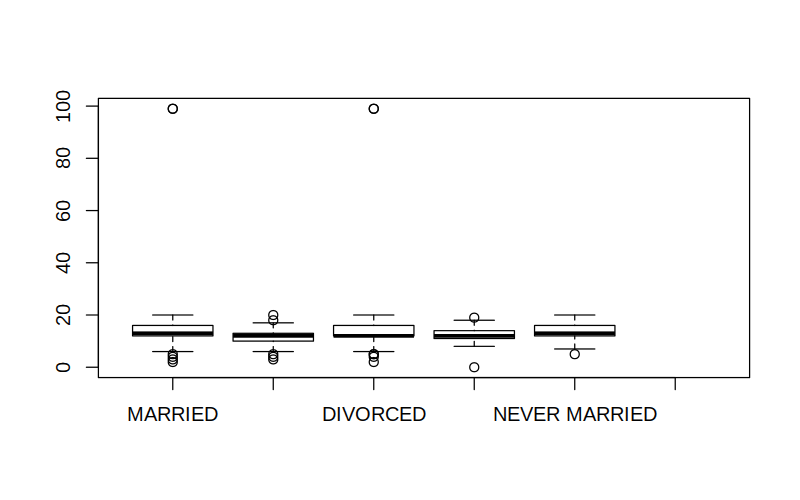
\includegraphics[width=.9\textwidth]{images/examplePlot2.png}
\end{block} \end{columns}
\end{frame}

\begin{frame}[fragile,label=sec-7-9]{Basic graphics: Mosaic chart}
 Thanks to classes and methods, you can \verb~plot()~ many kinds of objects:
\begin{columns} \column{.85\textwidth} \begin{block}{}
\begin{minted}[fontsize=\scriptsize]{r}
with(datGSS, # Plot factor X factor
     plot(marital, happy))
\end{minted}
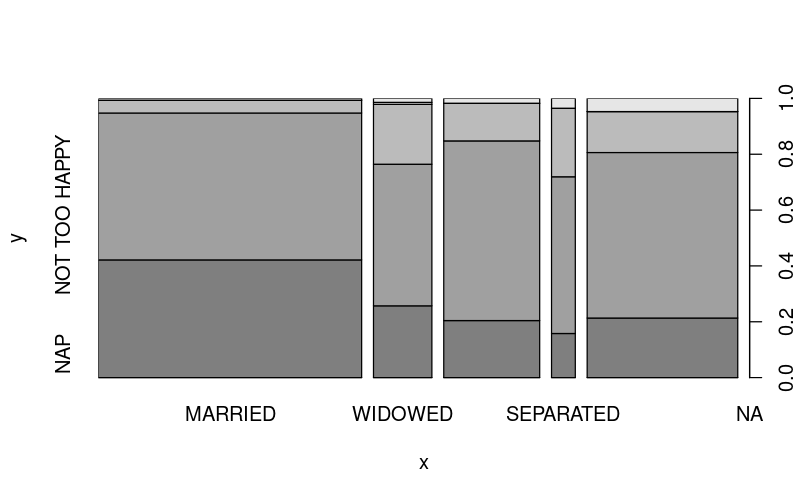
\includegraphics[width=.95\textwidth]{images/examplePlot3.png}

\end{block} \end{columns}
\end{frame}

\begin{frame}[label=sec-7-10]{Exercise 3}
Using the datGSS data.frame

\begin{enumerate}
\item Cross-tabulate sex and emailhrs
\item Calculate the mean and standard deviation of incomdol by sex
\item Save the results of the previous two calculations to a file
\item Create a scatter plot with educ on the x-axis and incomdol on the y-axis
\end{enumerate}
\end{frame}

\section{Wrap-up}
\label{sec-8}

\begin{frame}[label=sec-8-1]{Help us make this workshop better!}
\begin{itemize}
\item Please take a moment to fill out a very short feedback form

\item These workshops exist for you – tell us what you need!

\item \url{http://tinyurl.com/R-intro-feedback}
\end{itemize}
\end{frame}

\begin{frame}[label=sec-8-2]{Additional resources}
\begin{itemize}
\item IQSS workshops: \url{http://projects.iq.harvard.edu/rtc/filter_by/workshops}

\item IQSS statistical consulting: \url{http://rtc.iq.harvard.edu}

\item Software (all free!):
\begin{itemize}
\item R and R package download: \url{http://cran.r-project.org}
\item Rstudio download: \url{http://rstudio.org}
\item ESS (emacs R package): \url{http://ess.r-project.org/}
\end{itemize}

\item Online tutorials
\begin{itemize}
\item \url{http://www.codeschool.com/courses/try-r}
\item \url{http://www.datamind.org}
\end{itemize}

\item Getting help:
\begin{itemize}
\item Documentation and tutorials: \url{http://cran.r-project.org/other-docs.html}
\item Recommended R packages by topic: \url{http://cran.r-project.org/web/views/}
\item Mailing list: \url{https://stat.ethz.ch/mailman/listinfo/r-help}
\item StackOverflow: \url{http://stackoverflow.com/questions/tagged/r}
\end{itemize}
\end{itemize}
\end{frame}


\section{Exercise solutions}
\label{sec-9}

\begin{frame}[fragile,label=sec-9-1]{Exercise 0 solution}
 \begin{enumerate}
\setcounter{enumi}{0}
\item ] Try to get R to add 2 plus 2.
\end{enumerate}
\begin{minted}[fontsize=\scriptsize]{r}
2 + 2
\end{minted}

\begin{enumerate}
\setcounter{enumi}{1}
\item Try to figure out how evaluate lines directly from your R script.
\end{enumerate}
\texttt{In Rstudo this is 'Control-Enter'; may be different in another GUI}
\begin{enumerate}
\setcounter{enumi}{2}
\item R includes extensive documentation, including a file named "An introduction to R". Try to find this help file.
\end{enumerate}
\texttt{Go to the main help page by running 'help.start() or using the GUI menu, find and click on the link to "An Introduction to R".}
\begin{enumerate}
\setcounter{enumi}{3}
\item Go to \url{http://cran.r-project.org/web/views/} and skim the topic closest to your field/interests.
\end{enumerate}
\texttt{I like the machine learning topic!}
\end{frame}

\begin{frame}[fragile,label=sec-9-2]{Exercise 1 solution}
 \begin{enumerate}
\setcounter{enumi}{0}
\item Load the foreign package if you haven't already done so
\end{enumerate}
\begin{minted}[fontsize=\scriptsize]{r}
library(foreign)
\end{minted}

\begin{enumerate}
\setcounter{enumi}{1}
\item Look at the help page for the read.spss function
\end{enumerate}
\begin{minted}[fontsize=\scriptsize]{r}
help("read.spss")
\end{minted}

\begin{enumerate}
\setcounter{enumi}{2}
\item Read the SPSS data set in dataSets/gss.sav and assign the result to an R data object named GSS.sav
\end{enumerate}
\begin{minted}[fontsize=\scriptsize]{r}
gss.data <- read.spss("dataSets/gss.sav", to.data.frame=TRUE)
\end{minted}

\begin{enumerate}
\setcounter{enumi}{3}
\item Make sure that the data loaded in step 2 is a data.frame (hint: check the arguments documented in the help page)
\end{enumerate}
\begin{minted}[fontsize=\scriptsize]{r}
class(gss.data)
\end{minted}

\begin{enumerate}
\setcounter{enumi}{4}
\item Display the dimensions of the GSS.sav.
\end{enumerate}
\begin{minted}[fontsize=\scriptsize]{r}
dim(gss.data)
nrow(gss.data)
ncol(gss.data)
\end{minted}

\begin{enumerate}
\setcounter{enumi}{5}
\item BONUS: figure out how to read the Excel file "gss.xlsx" into R
\end{enumerate}
\begin{minted}[fontsize=\scriptsize]{r}
library(XLConnect)
dat <- readWorksheetFromFile("dataSets/gss.xlsx", sheet = 1)
class(dat); dim(dat)
\end{minted}
\end{frame}


\begin{frame}[fragile,label=sec-9-3]{Exercise 2 solution}
 Use the gss.rds data set
\begin{minted}[fontsize=\scriptsize]{r}
gss <- readRDS("dataSets/gss.rds")
\end{minted}

\begin{enumerate}
\setcounter{enumi}{0}
\item Create a subset of the data containing only rows where "usecomp" = "Yes". How many computer users are there?
\end{enumerate}
\begin{minted}[fontsize=\scriptsize]{r}
gss.usecomp <- subset(gss, usecomp == "Yes")
nrow(gss.usecomp)
\end{minted}

\begin{enumerate}
\setcounter{enumi}{1}
\item Generate the following variables:
\begin{itemize}
\item "rich" equal to 0 if rincdol is less than 100000, and 1 otherwise
\item "sinc" equal to incomdol - rincdol
\end{itemize}
\end{enumerate}
\begin{minted}[fontsize=\scriptsize]{r}
gss <- transform(gss,
                 rich = ifelse(rincdol < 100000, 0, 1),
                 sinc = incomdol - rincdol)
head(subset(gss, select = c("rincdol", "incomdol", "rich", "sinc")))
\end{minted}


\begin{enumerate}
\setcounter{enumi}{2}
\item Generate a variable named "dual.earn" equal to 1 if both wkftwife = 1 and wkfthusb = 1, and zero otherwise. How many dual earners are there?
\end{enumerate}
\begin{minted}[fontsize=\scriptsize]{r}
gss$dual.earn <- ifelse(gss$wkftwife == 1 & gss$wkfthusb == 1, 1, 0)
nrow(subset(gss, dual.earn == 1))
\end{minted}
\end{frame}

\begin{frame}[fragile,label=sec-9-4]{Exercise 3 solution}
 Using the datGSS data.frame

\begin{enumerate}
\setcounter{enumi}{0}
\item Cross-tabulate sex and emailhrs
\end{enumerate}
\begin{minted}[fontsize=\scriptsize]{r}
with(datGSS, table(sex, emailhrs))
\end{minted}

\begin{enumerate}
\setcounter{enumi}{1}
\item Calculate the mean and standard deviation of incomdol by sex
\end{enumerate}
\begin{minted}[fontsize=\scriptsize]{r}
by(datGSS$incomdol, datGSS$sex, mean)
by(datGSS$incomdol, datGSS$sex, sd)
\end{minted}

\begin{enumerate}
\setcounter{enumi}{2}
\item Create a scatter plot with educ on the x-axis and incomdol on the y-axis
\end{enumerate}
\begin{minted}[fontsize=\scriptsize]{r}
plot(subset(datGSS, select = c("educ", "incomdol")))
\end{minted}
\end{frame}
% Emacs 24.3.1 (Org mode 8.2.7c)
\end{document}